\documentclass[sigconf]{acmart}
\usepackage{tabulary}
\usepackage{booktabs}
%%
%% \BibTeX command to typeset BibTeX logo in the docs
\AtBeginDocument{%
  \providecommand\BibTeX{{%
    Bib\TeX}}}

%% Rights management information.  This information is sent to you
%% when you complete the rights form.  These commands have SAMPLE
%% values in them; it is your responsibility as an author to replace
%% the commands and values with those provided to you when you
%% complete the rights form.
\setcopyright{none}
\copyrightyear{2024}
\acmYear{2024}
\acmDOI{XXXXXXX.XXXXXXX}

%% These commands are for a PROCEEDINGS abstract or paper.
\acmConference[Data Mining Project '24]{Data Mining Project}{April 2024}{Boulder, CO}
%%
%%  Uncomment \acmBooktitle if the title of the proceedings is different
%%  from ``Proceedings of ...''!
%%
%%\acmBooktitle{Woodstock '18: ACM Symposium on Neural Gaze Detection,
%%  June 03--05, 2018, Woodstock, NY}
%% \acmISBN{978-1-4503-XXXX-X/18/06}

%%
%% Submission ID.
%% Use this when submitting an article to a sponsored event. You'll
%% receive a unique submission ID from the organizers
%% of the event, and this ID should be used as the parameter to this command.
%%\acmSubmissionID{123-A56-BU3}

%%
%% For managing citations, it is recommended to use bibliography
%% files in BibTeX format.
%%
%% You can then either use BibTeX with the ACM-Reference-Format style,
%% or BibLaTeX with the acmnumeric or acmauthoryear sytles, that include
%% support for advanced citation of software artefact from the
%% biblatex-software package, also separately available on CTAN.
%%
%% Look at the sample-*-biblatex.tex files for templates showcasing
%% the biblatex styles.
%%

%%
%% The majority of ACM publications use numbered citations and
%% references.  The command \citestyle{authoryear} switches to the
%% "author year" style.
%%
%% If you are preparing content for an event
%% sponsored by ACM SIGGRAPH, you must use the "author year" style of
%% citations and references.
%% Uncommenting
%% the next command will enable that style.
%%\citestyle{acmauthoryear}


%%
%% end of the preamble, start of the body of the document source.
\begin{document}

%%
%% The "title" command has an optional parameter,
%% allowing the author to define a "short title" to be used in page headers.
\title{Energy Grid Forecasting and Anomaly Detection}

%%
%% The "author" command and its associated commands are used to define
%% the authors and their affiliations.
%% Of note is the shared affiliation of the first two authors, and the
%% "authornote" and "authornotemark" commands
%% used to denote shared contribution to the research.

\author{Cody Hill}
\affiliation{%
  \institution{University of Colorado Boulder}
  \city{Boulder}
  \country{USA}}
\email{cody.hill-1@colorado.edu}


%%
%% By default, the full list of authors will be used in the page
%% headers. Often, this list is too long, and will overlap
%% other information printed in the page headers. This command allows
%% the author to define a more concise list
%% of authors' names for this purpose.
\renewcommand{\shortauthors}{C. Hill}

%%
%% The abstract is a short summary of the work to be presented in the
%% article.
\begin{abstract}
Energy forecasting is a vital part of today's energy markets and operations. It is used to set the cost of electricity, determine when power generation should be increased, and decide when power needs to be directed to or from other regions of the electrical grid. Electrical energy demand continues to rise, especially with the recent widespread adoption of electric vehicles and heat pumps. As a result, the electrical grid will need to become more robust and adaptive as this increase in demand comes in tandem with a transition away from fossil fuels and into a more diversified energy market and with it, more complex cycles. These circumstances make accurate forecasting and periodicity identification of electrical loads and generation that much more important, and it is necessary to research the differences in forecasting applications and relevance in various short-term, medium-term, and long-term settings.

Many of the statistical time series forecasting techniques of the past are still in use today, each with their own strengths and weaknesses, often trading compute efficiency with lesser accuracy in long-term forecast horizons or ability to capture multiple seasonal periods. More modern machine learning models and neural network-based architectures tend to generalize through forecasting horizons better, but often at great cost of compute resources making them inefficient for short forecast horizon forecasts. Though because of the potential for complexity of energy load patterns, both categories see benefits in task-specific tuning. By evaluating each forecasting model's accuracy across various context windows and forecasting horizons, this project presents a thorough comparison on which techniques are most relevant in the task-specific energy grid context and each forecast horizon.
\end{abstract}

%%
%% The code below is generated by the tool at http://dl.acm.org/ccs.cfm.
%% Please copy and paste the code instead of the example below.
%%
\begin{CCSXML}
<ccs2012>
   <concept>
       <concept_id>10002950.10003648.10003688.10003693</concept_id>
       <concept_desc>Mathematics of computing~Time series analysis</concept_desc>
       <concept_significance>500</concept_significance>
       </concept>
   <concept>
       <concept_id>10010147.10010257.10010258.10010259.10010264</concept_id>
       <concept_desc>Computing methodologies~Supervised learning by regression</concept_desc>
       <concept_significance>500</concept_significance>
       </concept>
   <concept>
       <concept_id>10010147.10010257.10010293.10003660</concept_id>
       <concept_desc>Computing methodologies~Classification and regression trees</concept_desc>
       <concept_significance>300</concept_significance>
       </concept>
   <concept>
       <concept_id>10010147.10010257.10010293.10010075.10010295</concept_id>
       <concept_desc>Computing methodologies~Support vector machines</concept_desc>
       <concept_significance>300</concept_significance>
       </concept>
   <concept>
       <concept_id>10010147.10010257.10010293.10010294</concept_id>
       <concept_desc>Computing methodologies~Neural networks</concept_desc>
       <concept_significance>300</concept_significance>
       </concept>
   <concept>
       <concept_id>10010405.10010481.10010487</concept_id>
       <concept_desc>Applied computing~Forecasting</concept_desc>
       <concept_significance>500</concept_significance>
       </concept>
 </ccs2012>
\end{CCSXML}

\ccsdesc[500]{Mathematics of computing~Time series analysis}
\ccsdesc[500]{Computing methodologies~Supervised learning by regression}
\ccsdesc[300]{Computing methodologies~Classification and regression trees}
\ccsdesc[300]{Computing methodologies~Support vector machines}
\ccsdesc[300]{Computing methodologies~Neural networks}
\ccsdesc[500]{Applied computing~Forecasting}

%%
%% Keywords. The author(s) should pick words that accurately describe
%% the work being presented. Separate the keywords with commas.
\keywords{time series forecasting, anomaly detection, energy load, renewables, energy grid}
%% A "teaser" image appears between the author and affiliation
%% information and the body of the document, and typically spans the
%% page.
\begin{teaserfigure}
  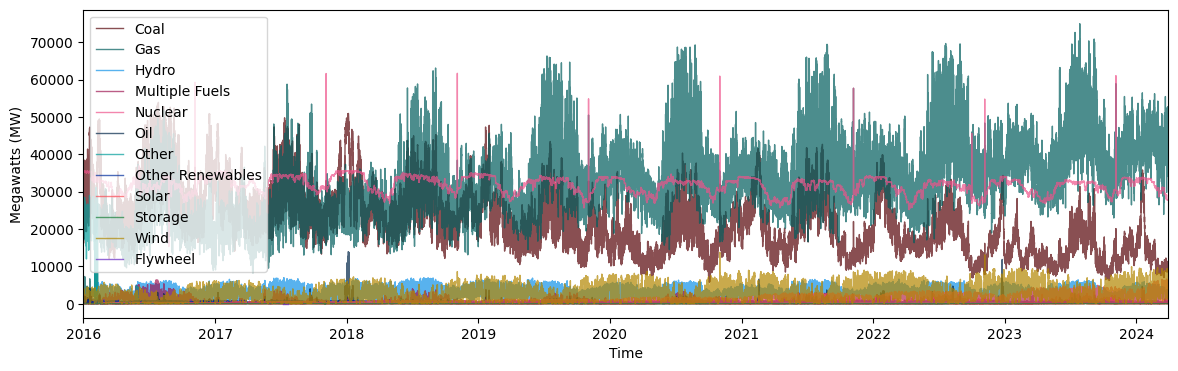
\includegraphics[width=\textwidth]{Images/Energy_Gen_Teaser.png}
  \caption{Energy Generated in Megawatts (MW) by Fuel Type.}
  \Description{}
  \label{fig:teaser}
\end{teaserfigure}

%%
%% This command processes the author and affiliation and title
%% information and builds the first part of the formatted document.
\maketitle

\section{Author's Note}
This document is to be used as a project proposal for the beginning planning stages of the project as well as a living-document as the project progresses. Up until project completion when a new version will be created to fill in the results.

\section{Introduction}
Energy forecasting is an important task to not only determine the expected load on the energy grid and the requirements of energy providers to meet that demand by either ramping up production or diverting sources altogether \cite{Hong16}. Identifying hourly, daily, seasonal, or even yearly energy demands accurately has substantial impact on not only the logistics of the infrastructure of our energy grid, but also the complex energy marketplace. These intervals, or forecast horizons, in the context of predictive models are defined in Table 1. Short-term forecasts can be useful for players in power markets where prices dynamically shift based on generation supply, customer demand, and financial spot and derivative contracts which are all based on energy forecasting \cite{Bunn04}. Very short-term forecasts can be important for power distributors and operators that want to meet customer demands more efficiently. Long-term forecasts are important in infrastructure planning and energy provider and distributers long-term planning. An example of a long-term forecast can be seen in Figure 2.

In the past this predictive role was largely upheld with statistical point-estimate models, but with the growth of our predictive models along with the diversification of the energy grid, more modern probabilistic interval forecasting techniques have begun to be used \cite{Lee21, Weron14, Hong16}. This diversification of the energy grid not only comes from energy reforms by way of deregulating the national electric market in the 1990's, but emerging cultural desires and improved technology in renewable energies, driving a need for a better electrical grid \cite{Joskow01}.

  \begin{figure}[hbt!]
    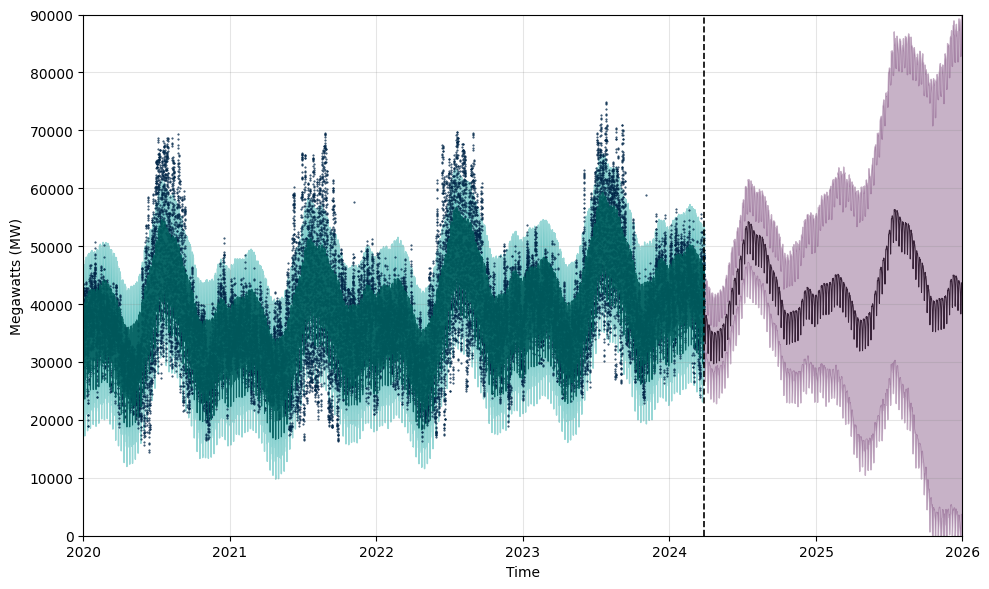
\includegraphics[width=\columnwidth]{Images/Forecast.png}
    \caption{Long-Term Forecast of Natural Gas Energy Generation Using Meta's Prophet Model. Actual observations are represented by the blue points, forecasted fit and predictions are in teal and purple respectively.}
    \Description{}
    \label{fig:forecast}
  \end{figure}

Electricity generation has always been mostly an on-demand industry and largely continues to be, where the energy we generate needs to be transmitted and used within a short period of time because we lack efficient systems for energy storage at scale \cite{Lai21}. This fact presents additional complications when many renewable energies only produce energy in certain conditions, making its effective use more reliant on forecasting to navigate a more diverse and complex power grid. Additionally, with the cultural and regulatory push towards end-users adopting the use of electric appliances, electric vehicles, and heat pumps, energy demand will continue to change \cite{Archsmith22}. These circumstances mean accurate forecasting is becoming even more important with improvements having the potential to better reduce reliance on fossil-fuel energies by more efficiently filling in gaps of energy demands with a more diversified and efficient energy grid.

\begin{table}
\centering
\caption{Defining prediction forecast horizon intervals. The forecast horizon determines how far into the future a forecast model predicts.}
\begin{tabular}{clc}
\toprule
\hfill \textbf{No}. & \hfil \textbf{Forecast Horizon Intervals} & \textbf{Duration}\\
\cmidrule(lr){1-1}\cmidrule(rl){2-2}\cmidrule(rl){3-3}
  1 & Very Short-Term & $ X < $ 1 Hour \\
  2 & Short-Term  & 1 Hour $ \leq X < $ 1 Week  \\   
  3 & Medium-Term & 1 Week $ < X \leq $ 1 Year  \\   
  4 & Long-Term & $ X > $ 1 Year  \\ 
  \bottomrule
\end{tabular}
\end{table}

There is little consensus among researchers and professionals about what exemplifies state-of-the-art in time series forecasting. This seems to be due to many things including that time series forecasting is heavily task-specific, meaning one model may perform well with one type of data and forecast horizon, but might perform poorly when compared to other techniques with a different horizon or data type \cite{Yue21}. This is why it is still important to experiment and compare forecasting techniques on domain-specific time series data.

\section{Related Work}
Seasonal Autoregressive Integrated Moving Average (SARIMA) and Exponential Smoothing models tend to be useful in short and medium-term forecasts but can experience limitations modeling complex periodicity and interactions \cite{Muzaffar19, Hopf23}. Newer, but certainly not state-of-the-art, machine learning techniques such as Support Vector Machines, XGBoost, and a variety of Long Short-Term Memory (LSTM) network architectures tend to generalize better and excel across multiple forecast horizons \cite{Sun22, Muzaffar19}.

Hybrid models and ensemble methods, utilizing a variety of preprocessing techniques and combining models into a unified framework, are becoming more popular as of late. The process typically involves splitting the job of extracting different types of features from the data, say the temporal and spatial relationships of the time series, and feeding those outputs into yet another separate model to perform the forecasting \cite{Hua23}. This technique combines the strengths of multiple models resulting in improved results across all forecast horizons \cite{Hua23, Hopf23}. Many of these still utilize LSTM layers as their attention mechanism \cite{Sun22}.

Transformer-based models and other frameworks developed and popularized in the Large Language Model (LLM) space have found a foothold in time series forecasting in the last few years as well, but their use in time series forecasting is still being researched \cite{Zeng22}. Similar to the LSTM, transformer-based models capture complex context and relationships in data, but across greater distances of the training corpus with increased efficiency because of their ability to be parallelized effectively \cite{Zheng24}. This type of model benefits from pre-training on a large corpus of diverse data which simply does not exist in the public domain for time series data \cite{Hug24}. With more time and data, researchers believe transformer-based models can be effective at time series forecasting \cite{Hug24, Zheng24}.

\section{Methods and Proposed Work}
Several models stemming from different statistical and machine-learning families will be trained to perform electricity load forecasting across the different forecast horizon intervals listed in Table 1. Each model's amount of compute required for training and evaluation scores will be compared across different forecast horizons. See evaluation section for more details on the specific metrics used.

  \subsection{Data}
  Electric load data was collected by the Pennsylvania-New Jersey-Maryland Interconnection (PJM). PJM is a regional electrical transmission organization which coordinates electricity transmission in all or parts of Delaware, Illinois, Indiana, Kentucky, Maryland, Michigan, New Jersey, North Carolina, Ohio, Pennsylvania, Tennessee, Virginia, West Virginia, and the District of Columbia \cite{PJMZone24}. A map of this can bee seen in Figure 3.
  
  Weather data was retrieved from the National Oceanic and Atmospheric Administration's (NOAA) Regional Climate Center (RCC) Applied Climate Information System (ACIS) \cite{ACIS}. The data was manually downloaded by selecting a weather station and choosing relevant dates and features with the daily data listings form. 
  
  \begin{table}[hbt!]
\centering
\caption{Dataset size and date ranges.}
\begin{tabular}{lrl}
\toprule
\textbf{Dataset} & \hfil \textbf{Size (Rows)} & \textbf{Date Range} \\
\cmidrule(rl){1-1}\cmidrule(rl){2-2}\cmidrule(rl){3-3}
  Hourly Load & 5,446,243 & 1993/01/01 - 2024/03/27 \\
  Daily Weather & 32,400 & 1993/01/01 - 2024/04/09  \\   
  \bottomrule
\end{tabular}
\end{table}
  
  The electric load data sourced from PJM is a set of hourly load in megawatt-hours verified by the individual electric distribution companies \cite{PJMLoad24}. The hourly load data is flagged with geographical location data which will be leveraged to include regional weather data as a covariate in the models. 
  
  The weather data has a daily sample frequency which was the only data available at the time. Hourly data would have been preferable to match the frequency of the load data, but even at the mismatched sample rate, will be a valuable exogenous covariate. Features included in this dataset are the maximum and minimum recorded temperature, average temperature, precipitation in inches. 
  
  After data discovery, 5 zones were chosen for their sample size, variety in signal shape, and data continuity. The weather data was selected to match the zones of interest from the load dataset and along with the zone map in Figure 3, weather stations were chosen for each zone. The weather stations chosen to represent each zone were chosen under the following criteria: 1.) Weather station is geographically central to the zone. 2.) Weather station uptime and reliability (airport weather stations often chosen for this quality).
  
  An overview of the datasets can be seen in Table 2.
  
  \begin{figure}
    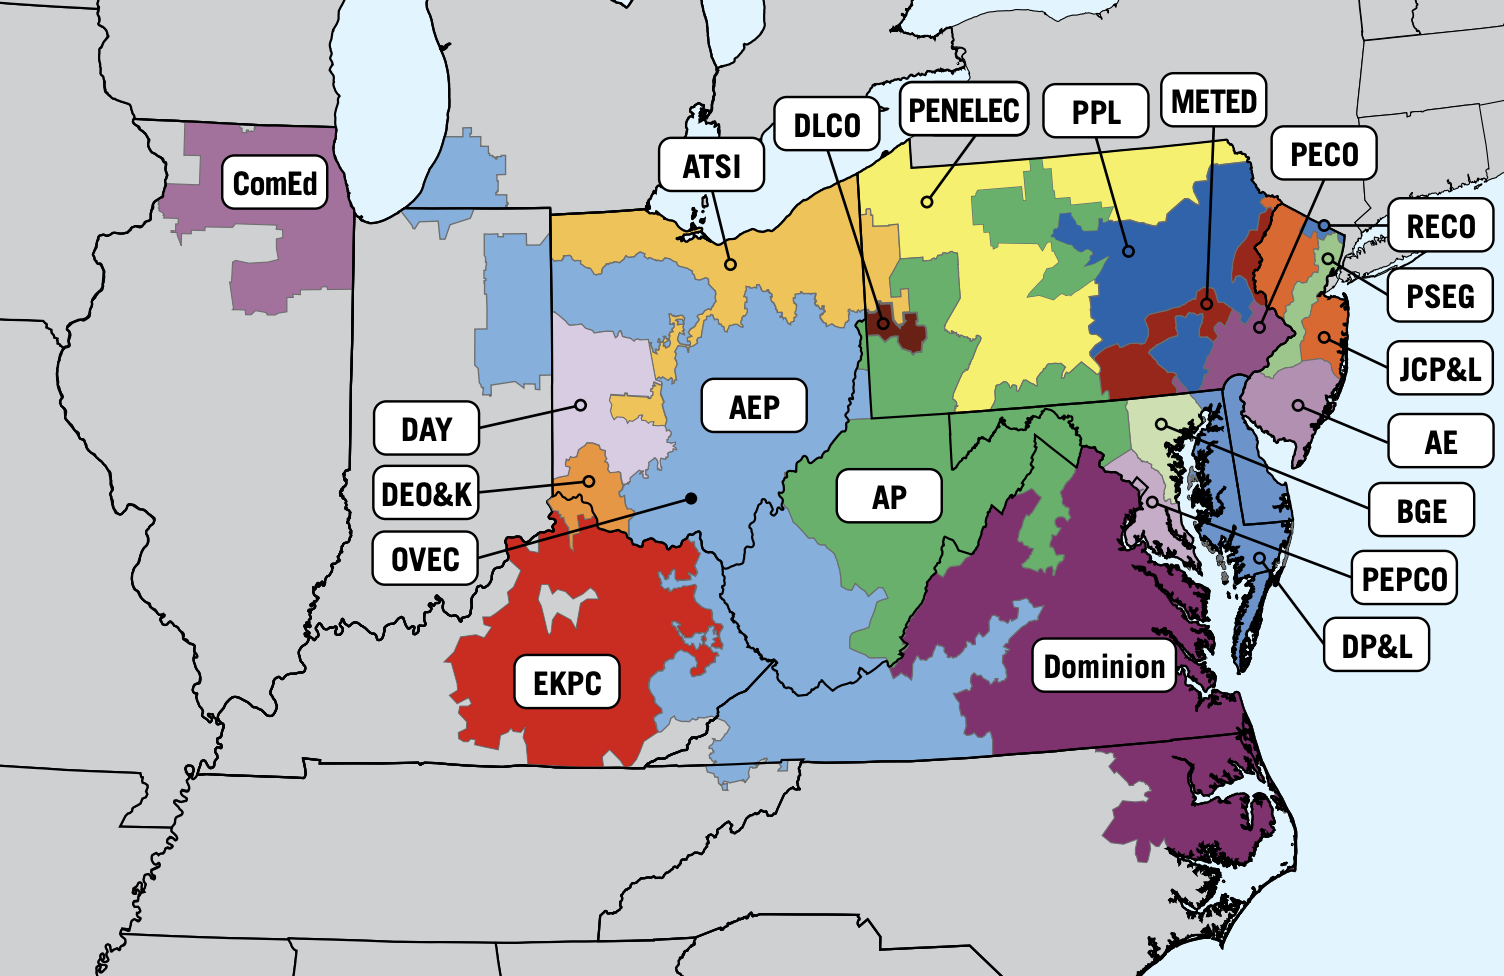
\includegraphics[width=\columnwidth]{Images/Zones.png}
    \caption{Regional Transmission Zones Labeled by Distributor IDs \protect \cite{PJM24}.}
    \Description{}
    \label{fig:zone}
  \end{figure}

  \subsection{Preprocessing}
  The electrical load data is retrieved from PJM's Data Miner 2 and each year is downloaded into a .csv file. These .csv files are then zipped so they can be pushed to github. All data is important into Pandas dataframes as it will allow all the following data transformations to be frictionless. Also, since several different models will be used, Pandas allows us to easily reformat the data between float arrays, tensors, and otherwise.
  
  The first step in preprocessing the datasets will be checking for any missing dates. Any missing rows will added by inserting the average value of the two surrounding observed data. Then the data will be analyzed for outliers, using a tumbling window method, replacing any identified outliers with the median of the window size. The two datasets will then be date aligned and merged.
  
    \subsection{Feature Engineering}
  Feature engineering is a large part of time series forecasting, typically past values of the target variable are highly correlated to future values. Several methods will be used to generate covariates that either have a signal smoothing effect, identifies seasonal periods, or encodes exogenous information.
  \begin{enumerate}
  \item \textbf{Date features} will be encoded in categorical features representing Hours, Days, Months, Years, and Day of Year - this will help the models identify recurring temporal relationships, or seasonality, in the target variable.
  \item \textbf{Rolling mean} of the target variable of the previous 1 month of data points, adding the rolling mean helps smooth out the signal, increasing model performance. 
  \item \textbf{Lagged features} at specific intervals are useful if an effort is made to match known seasonal periods within the data. Lagged features of the target variable at 1 hour, 6 hours, 24 hours, 1 week, and 1 month will be used. \textit{Note, a 1 year lagged feature would also be effective, but would have null values for the first year which can be problematic for some models and those rows would need to be removed.}
  \item \textbf{Fourier transform spectral density}, similar to lagged features, helps identify correlated seasonal periods. By performing the Fast Fourier Transform on the target variable and taking the absolute value of it, the most relevant seasonal frequencies will have the greatest magnitudes. An example of the resulting spectral density plot can be seen in Figure 4.
  
    \begin{figure}[hbt!]
    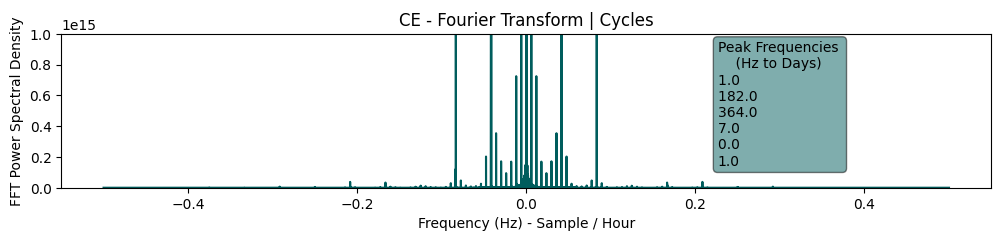
\includegraphics[width=\linewidth]{Images/FFT_Plot.png}
    \caption{Fourier transform spectral density plot of the ComEd (CE) zone. To cast frequency units to days: $\frac{1}{freq*24}$.}
    \Description{}
    \label{fig:fft}
  \end{figure}
  
  \item \textbf{First and Second-Order Derivatives/Differencing} finds the instantaneous rate of change between two observed data points and the acceleration of the rate of change respectively. This encodes direction, magnitude, and change of direction in time series data. An example plot of both orders of derivatives can be seen in Figure 7 in the appendix.
\end{enumerate}

Specific intervals of features such as lag, rolling mean, derivatives need to be considered carefully when used as exogenous features calculated from the target variable. This can be a great source of data leakage into the testing set if these are not data you would have in a prediction setting. One method to overcome this is to take a naive approach and assign last season's values. Another is to create a hybrid model which forecasts the exogenous features to include in the forecast. Finally, a rolling forecast can be used predict new datapoints and retrain the model with those predictions up until the intended forecast horizon is achieved. Here, the shorter length interval features will be excluded to prevent data leakage, but will remain implemented but not included as an exercise in time series feature engineering.

  \subsection{Tools and Techniques}
    The load data will then be analyzed and plotted for historical trends and to identify periodicity (cycles) at different context window intervals which will help set model expectations for the various forecast horizons. 
    
    Models of varying complexity and methodology will be used to better represent the broad spectrum of techniques used today, in an attempt to capture a good representation of which contemporary models work best for different forecast horizons. 

\textbf{Proposed models}:
\\
\textbf{Baseline}
\begin{itemize}
    \item{Seasonal Naive Forecast Model}
    \item{Mean}
\end{itemize}
\textbf{Statistical}
\begin{itemize}
    \item{Seasonal Autoregressive Integrated Moving Average (SARIMA)}
    \item{Multiple Seasonal-Trend decomposition using LOESS (MSTL)}
\end{itemize}
\textbf{Machine Learning}
\begin{itemize}
    \item{Support Vector Machine (SVM)}
    \item{XGBoost}
\end{itemize}
\textbf{Deep Learning}
\begin{itemize}
    \item{Temporal Fusion Transformers (TFT)}
\end{itemize}

Some models may require data transformation or normalization to perform effectively. For example, the SVM and TFT increase performance with scaled feature matrices. $$Z = \frac{(X - \bar{X})}{S}$$ 
Centers inputs around 0 with the sample mean, and scales them with the sample standard deviation.

\section{Evaluation}

\subsection{Training, Validation, and Testing Data Split}
The data will be split into a training, validation, testing split. A validation set is necessary here because several of the proposed forecasting models will require hyperparameter tuning. Once the data has been aggregated, cleaned, and finalized the exact ratio may be adjusted to ensure the test set is large enough to span the largest forecast horizon at least one or several times, depending on what is feasible with the data on hand.

  \begin{figure}[hbt!]
    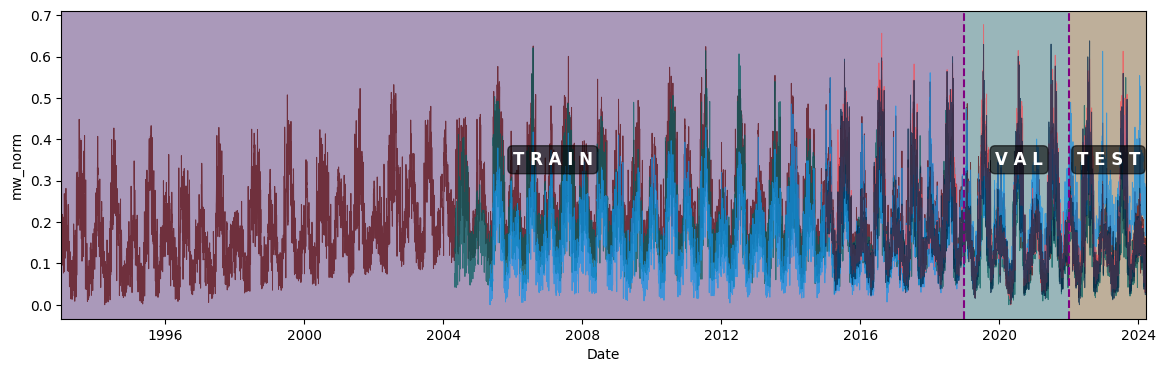
\includegraphics[width=\columnwidth]{Images/Split_Plot.png}
    \caption{Plot of the training, validation, and testing split.}
    \Description{}
    \label{fig:split}
  \end{figure}
 
To avoid data leakage and maintaining temporal relationships, the test set will always be assigned the most recent dates with zero overlap in the training or validation sets. Also, it is ensured that each set contains a reasonable amount of each periodicity. Details about the resulting split can be seen in Table 3 and Figure 5.


  \begin{table}[hbt!]
\centering
\caption{Dataset size and date ranges.}
\begin{tabular}{ll}
\toprule
\textbf{Split Set} & \textbf{Date Range} \\
\cmidrule(rl){1-1}\cmidrule(rl){2-2}
  Training & 1993/01/01 - 2018/12/31 \\
  Validation & 2019/01/01 - 2021/12/31  \\   
  Testing & 2022/01/01 - 2024/03/27  \\   
  \bottomrule
\end{tabular}
\end{table}

\subsection{Metrics}
Symmetric Mean Absolute Percentage Error (sMAPE) will be the evaluation metric used to compare all models. This will ensure comparisons of error across different models and forecasting horizons are normalized. 

\begin{equation}
\text{sMAPE} =\frac{200}{n}\sum_{i=1}^{n}\frac{\lvert y_i - \hat{y_i} \rvert}{\lvert y_i \rvert + \lvert \hat{y_i} \rvert}
\end{equation}

where $y_i$ and $\hat{y_i}$ are the actual values and forecasted values respectively, and $n$ is the number of points in the set.

One possible limitation of sMAPE is if a predicted value or actual value equals zero, the metric balloons to the maximum error value, and if both equals zero, the metric is undefined. Chosen evaluation metrics often have strengths and weaknesses, and it is yet unclear if this limitation will occur here.

Root Mean Squared Error (RMSE) will also be used in model evaluation to complement sMAPE. The value of including RMSE is that it is an easily interpretable quantitative metric resulting in a value that is in the same unit as the response. It also heavily penalizes predictions the further they are from the actual value.

\begin{equation}
\text{RMSE} =\sqrt\frac{\sum_{i=1}^{n}(y_i - \hat{y_i})^2}{n}
\end{equation}

where $y_i$ and $\hat{y_i}$ are the actual values and forecasted values respectively, and $n$ is the number of points in the set.

In conjunction with the RMSE, a Normalized RMSE (NRMSE) will also be used to compare models between zones, since each zone have varying scales of the target variable.

\begin{equation}
\text{NRMSE} = \frac{RMSE}{\bar{Y}}
\end{equation}

where $\bar{Y}$ is the mean of the actual values.

\section{Discussion}

After data discovery and feature engineering, during the preliminary model setup it was determined a few of the proposed models would not be moving forward to testing due to the size of the dataset and feature matrix. The ARIMA-based models, even when specified as univariate models, require substantial setup and tuning which on the machine it was being worked on became untenable. Train times for this and a few neural-network models, even with reduced training set sizes, were not able to be completed due to hardware limitations. Unfortunately these models will not move forward or will be reduced in scope at some level. These reductions and scope will be listed per model as they arise. However, this does add justification to the thesis that forecast horizon lengths and models need to be chosen at a task-specific level because lengthy training durations on short forecast horizon lengths heavily outweigh the tradeoff balance.

More discussions and analysis will be added here when the project has been completed.

\subsection{Project Timeline}

Table 4 outlines the specific tasks and their projected schedule.

\begin{table}[hbt!]
\centering
\caption{A general framework onto which the project will progress. This timeline is subject to change.}
\begin{tabular}{ll | c | c}
\toprule
\textbf{Timeline} & \textbf{Agenda Item} & \hfil \textbf{Progress} & \hfil \textbf{Done} \\
\cmidrule(rl){1-1}\cmidrule(rl){2-2}\cmidrule(rl){3-3}\cmidrule(rl){4-4}
  Days 1 - 5 & Data Mining & \textbf{--} & \textbf{X} \\
  \cmidrule(rl){1-4}
   & \hspace{3mm}Hourly Load Data & -- & \textbf{X} \\   
   & \hspace{3mm}Hourly Generation Data & -- & \textbf{X} \\   
   & \hspace{3mm}Weather Data & \textbf{--} & \textbf{X}\\   
   & Cleaning/Preprocessing & \textbf{--} & \textbf{X}\\  
   \cmidrule(rl){2-4} 
   & \hspace{3mm}Datetime Alignment & \textbf{--} & \textbf{X}\\   
   & \hspace{3mm}Aggregate by Zones & \textbf{--} & \textbf{X}\\   
   & \hspace{3mm}Outlier Inspection & \textbf{--} & \textbf{X}\\   
   & \hspace{3mm}Corrupted Data Removal & \textbf{--} & \textbf{X}\\  
   & Feature Engineering & \textbf{--} & \textbf{X}\\  
   & Exploratory Data Analysis & \textbf{--} & \textbf{X}\\  
   \cmidrule(rl){2-4} 
   & Train/Val/Test Split &\textbf{--} & \textbf{X}\\  
   \cmidrule(rl){2-4} 
  Days 6-8 & Anomaly Detection & & \\  
   \cmidrule(rl){1-4} 
   & Forecast Model Setup &\textbf{--} & \textbf{X}\\  
   \cmidrule(rl){2-4} 
   & \hspace{3mm}Training &\textbf{--} & \textbf{X} \\  
   & \hspace{3mm}Val. Optimizations &\textbf{--} & \textbf{X}\\  
   & Build Eval. Functions & \textbf{X}& \\  
   \cmidrule(rl){2-4} 
  Days 9-10 & Test Results & & \\  
  \cmidrule(rl){1-4} 
   & Discussion & & \\
   \cmidrule(rl){2-4}   
   & Conclusion & & \\  
   \cmidrule(rl){2-4} 
  \bottomrule
\end{tabular}
\end{table}

\subsection{Potential Challenges}
A few challenges may arise impeding progress or causing the project to fall behind schedule are expected to be the following. 
Generally, properly fitting the data to the number of proposed forecast models within the timeline may pose a challenge. Specifically, the neural-network architectures can take considerable time to build from the ground up without intimate knowledge and experience of their specific architectures. Also, completely fleshing out the three goals of the project on schedule may be cause for concern and need reevaluation -- anomaly detection, hourly load forecasting, and hourly energy generation forecasting.

The granularity of the data may post issues in accurately forecasting the shorter forecast horizons. Since all collected data has a time-step (sample rate) granularity of one hour, predictions less than one hour have little basis in reality. Data with smaller a time-step would be required for accurate shorter forecast horizons.

\subsection{Alternate Approaches}
If the project is running behind the timeline a few different approaches can be considered to make the target deadlines. 

\begin{enumerate}
  \item The number of models can be reduced but leaving at least one remaining from each model type. 
  \item In the case of some of the neural-network based architectures and machine-learning approaches, complexity can be reduced by utilizing more out-of-the-box approaches/models. 
  \item Instead of forecasting both hourly load usage and generation by fuel type, the scope of the project can be reduced to focus on just one of these domains.
  \item Further reduce the scope to solely focus on anomaly detection.
\end{enumerate}

\section{Results}
As the other models are still being worked on here is a preliminary look at the results for the baseline models and XGBoost which has been tuned and finalized.

Preliminary Results:
  \begin{figure}[hbt!]
    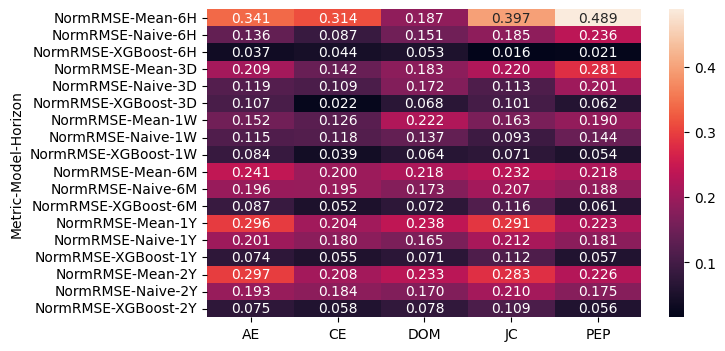
\includegraphics[width=\columnwidth]{Images/Prelim_Results.png}
    \caption{Results of the models that are completed.}
    \Description{}
    \label{fig:results}
  \end{figure}

\section{Conclusion}
By analyzing and modeling energy time series data we can efficiently and accurately forecast into the future different interval forecast horizons, which correspond to real-world decisions. Depending on the time-scale in which those decisions rely, analysts must appropriately identify what side of the accuracy and efficiency tradeoff is more important in their use case. Modern techniques in time series forecasting have reduced the errors in all forecast horizon intervals and continue to generalize those prediction abilities across many domains, but many of the most accurate models take a considerable amount of time or hardware to train. This type of research and technology is necessary for uninterrupted energy generation and distribution due to the ever-increasing demands and complexity of our energy grids.

\subsection{Key Findings}
XGBoost performs surprisingly well in this domain at many forecast horizons, greatly improving over the baseline methods. On top of its performance the computational demands are very low and training takes negligible time compared to other machine learning and neural network-based methods.

Once the remaining models are completed, a further comparative analysis across all horizons and methods can be completed.
\subsection{Future Work}
To be completed upon project completion.

\section{Appendices}

  \begin{figure}[hbt!]
    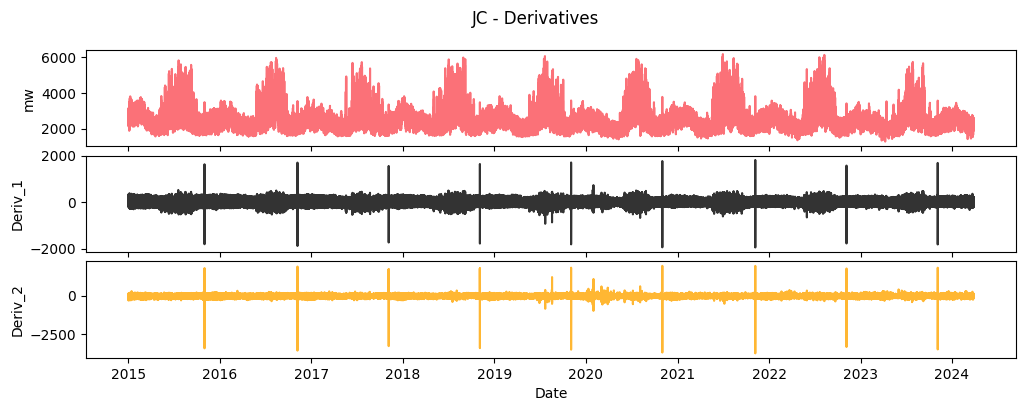
\includegraphics[width=\columnwidth]{Images/Deriv_Plot.png}
    \caption{First and second-order derivatives/differencing of Megawatts in black and yellow respectively.}
    \Description{}
    \label{fig:deriv}
  \end{figure}


%%
%% The acknowledgments section is defined using the "acks" environment
%% (and NOT an unnumbered section). This ensures the proper
%% identification of the section in the article metadata, and the
%% consistent spelling of the heading.
\begin{acks}
 \hspace{3mm} Sqyd, for always brewing the morning coffee -- I know it's 8 cups of water, now.

Luna, for breaking up the hyper-focused monotony with mind-clearing afternoon walks.
\end{acks}

%%
%% The next two lines define the bibliography style to be used, and
%% the bibliography file.
\bibliographystyle{ACM-Reference-Format}
\bibliography{References_Checkpoint}


%%
%% If your work has an appendix, this is the place to put it.
\appendix

\end{document}
\endinput
%%
%% End of file `sample-sigconf.tex'.
